%Préambule du document :
\documentclass[12pt, a4paper]{book}
%\usepackage[latin1]{inputenc} 
\usepackage[utf8]{inputenc} % accents
\usepackage{gensymb} % degree symbol ° (\degree)
\usepackage[T1]{fontenc} % | "`pipe"' character
\usepackage{graphicx}
\usepackage{titling}
\usepackage{amssymb} 
\usepackage{minitoc} % chapter's tocs
\usepackage{authblk} % author affiliations
\usepackage{fancyhdr} % modify the headers
\usepackage{tabularx} % tables not larger than A4
\usepackage[table]{xcolor} %colors inside the tables
\usepackage{float}
\usepackage{multicol} % multiple columns in some sections
\usepackage[inner=2cm,outer=2cm]{geometry} %A4 margins
\usepackage{siunitx}
\usepackage[labelfont=bf, margin=0.5cm]{caption} % for figure captions in minipages
\usepackage{hyperref} %link references (toc, citations) inside document
\usepackage{natbib} % to cite with parentheses and plain text et only year if you please...
\usepackage{amsmath}
 \usepackage{fixltx2e} % allows overrightarrow to be in caption
 \MakeRobust{\overrightarrow}


\bibliographystyle{plainnat} % reference style
\renewcommand{\bibname}{References} %Rename "`bibliography"' => "`references"'
\newcommand*{\doi}[1]{\href{https://doi.org/#1}{doi: #1}}


\hypersetup{
    colorlinks,
    citecolor=brown,
    filecolor=green,
    linkcolor=red,
    urlcolor=blue
}
\hypersetup{linktocpage}


\pagestyle{fancy}
\fancyhead{}
\fancyfoot{}
\fancyhead[RO,LE]{\thepage}
\fancyhead[LO]{\leftmark}
\fancyhead[RE]{\rightmark}
\setcounter{tocdepth}{1} % we only want chapters and sections in toc
\setcounter{minitocdepth}{2} %we want sections and subsections in chapters' minitocs

\pretitle{%
  \begin{center}
  
  
\includegraphics[width=17cm]{../Logo_software.png}\\[\bigskipamount]
}
\posttitle{
\\
  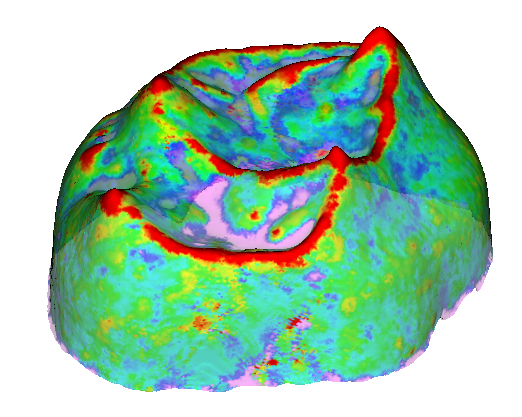
\includegraphics[width=8cm]{tutorial09.png}\\[\bigskipamount]
\end{center}}

%\postdate{
%
\includegraphics[width=15cm]{logo_affiliations.png}
%}

\title{Tutorial 09: curvature, scalar smoothing and normalization}



%\titlepicture[width=13cm]{Logo_software.png}
\author{Renaud LEBRUN}
\affil{Institut des Sciences de l'Evolution, Université de Montpellier, France}
\date{\today} 

\def\chaptername{Tutorial}
\setcounter{chapter}{9}
%Corps du document :
\begin{document}

	\dominitoc

\maketitle


\faketableofcontents

%\chapter{Working with landmarks}
\addstarredchapter{Thickness between objects}

\markboth{Tutorial 09: curvature, scalar smoothing and normalization}{}

\minitoc 
Tutorial 09 includes:
\begin{itemize}
\item One .ntw (MorphoDig project) file
\item One .vtk surface files representing the Enamel Dentine Junction (EDJ) of a Neolithic human upper left second molar.
\item One .pos (position) files 
\item The present .pdf document
\end{itemize}



\section{About the specimen}
The 3D model corresponds to a virtually reconstructed Enamel-Dentine Junction (EDJ) of a left upper permanent second molars (LUM2) from a Neolithic human of the necropolis of Gurgy (France). This specimen (GLN04-201-ULM2) was published in \citet{LeLuyer2016}, and the 3D model was released in \citet{LeLuyer2016a}.
The 3D data were obtained by computerized microtomography at the MRI \si{\micro}CT platform housed at the ISEM. 


\section{A brief overview of enclosed files}
		
The present tutorial contains a project .ntw file, which is useful to open the EDJ surface in a convenient position. Open the enclosed .ntw file (File->Open Project, then select "Enamel\_thickness.ntw"). Once loaded, the two surfaces are opened, are given the positions enclosed in the two position files, and a color. Note that the newly opened surfaces are unselected.


\section{Tutorial}

\subsection{Curvature}
The EDJ 3D representation already contains 4 "Curvature" scalar arrays: Curvature\_mean, Curvature\_min, Curvature\_max, Curvature\_gaussian.\\ 
The curvature dialog can be opened by clicking on Scalars->Compute curvature for each selected surface (see Fig. \ref{curvature_dialog} \pageref{curvature_dialog}). These arrays were computed using the vtkCurvatures filter.\\
The vtkCurvatures filter offers 4 ways to compute surface's
curvature at each vertex. :\\
- Principal maximal curvature\\
- Principal minimal curvature\\
- Gaussian curvature\\
- Mean curvature.\\

\begin{figure}
  \centering
  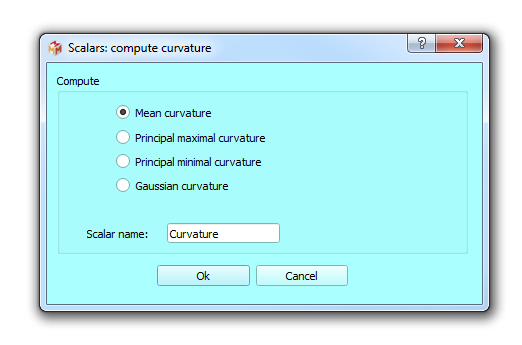
\includegraphics[scale=0.5]{curvature_dialog.png} 
	\caption{Curvature dialog.}
\label{curvature_dialog}
 
\subsection{Smoothing}
The 4 "Curvature" scalar arrays (Curvature\_mean, Curvature\_min, Curvature\_max, Curvature\_gaussian) contain a lot of noise. In order to reduce noise and retrieve more biologically relevant information, scalars can be "smoothed" in different ways (see \ref{smoothing_scalars_dialog}). In our case, for each vertex, all "vertices closer than surface average size/40" were retrieved, and the smooth output was computed as the median of the scalar values found for all found neighbor vertices.

\begin{figure}
  \centering
  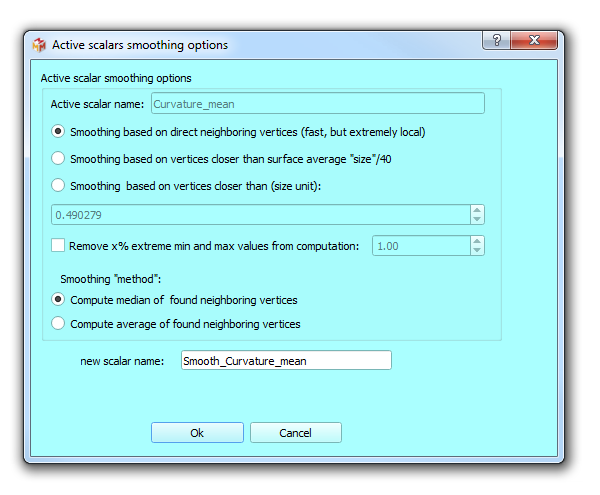
\includegraphics[scale=0.5]{scalar_smoothing_dialog.png} 
	\caption{ 
Scalar smoothing dialog. Smoothing can be computed using only direct neighbor vertices. A much larger area can also be investigated to produce a "smoothed" output. A percentage of extreme minimal and maximal values found can be excluded from the smoothing process. Also, the "smoothed" output can be computed as the average or as the median of the scalar values found for the neighbor vertices.
	}
\label{smoothing_scalars_dialog}
\end{figure}

\subsection{Normalization}

\section{Acknowledgements}
MicroCT data acquisition was funded by the Research National Agency through the DHP project (dir: S. Rottier; 2012-14; Université Bordeaux 1/LaScArBx; Grant number: ANR-10-LABX-52) and the PEPS 3Dent’in (dir: P. Bayle; 2013-14; PEPS IdEx Bordeaux/CNRS; Grant number: ANR-10-IDEX-03-02). M. Le Luyer, who performed 3D data acquisition, benefited from a doctoral grant of the Ministère de l’Enseignement Supérieur et de la Recherche. MicroCT data presented in this work were produced through the technical facilities of the MRI platform and of the labEx CeMEB.


%\nocite{*}   % All bibliography items appear without citation in the text

%\cleardoublepage
%\phantomsection

\addcontentsline{toc}{section}{References}
\bibliography{References}	

\end{document} 

